\chapter{A study of graphs with calculus}
\label{sec:calculus-and-geometry}

\section{Invitation: sketching mountain ranges}

If I told you to \emph{sketch} out $x^2$, it'd be easy, right? Just a simple parabola would do. But if I say: plot $x^4 - 2x^3 + x^2 - x + 1$? It isn't so easy now is it. You could substitute various $x$ and plot it into the graph directly. But I'm asking for a rough sketch, not a plot. I just want the general shape and structure of the function: where are the highest and lowest points, the $x$-intercept, and the $y$-intercept. We're going to learn how to do exactly that in this chapter.

Imagine a function as a vast mountain range. When sketching this landscape, we're interested in identifying its peaks, valleys, and plateaus. A peak represents the sharp summit of a mountain, where the land falls away in all directions; a valley is a sunken area, nestled lower than the surrounding terrain; and a plateau is a level stretch, a temporary calm before the ascent resumes toward higher peaks or descends into deeper valleys. Standing at a peak, the land around you dips downward. In contrast, in a valley, everything rises above you. On a plateau, the ground is flat under your feet, but when gazed into the distance, one side raises higher, but the other reveals the path down. These important features are all characterized by a flat ground: a place with zero slope. If the mountain range represents function, then all of these points have zero first derivative.

Still, the information about zero first derivative is not sufficient to determine whether the point is a peak, a valley, or a plateau. What helps classify these points is the sign of the second derivative.

The second derivative suggest the concavity of a graph at that point. If the first derivative gives you the slope, the second derivative will give you the rate of change of that slope. If the second derivative is positive, it means that the function is increasing around that point; thus, that point must be a valley. If it's negative, then everything is decreasing around; thus, it's a peak. If it's zero, it's simply a plateau.

Just like a mountain, a function can have many points that has zero derivatives. Functions with more than one peaks exists. The first derivative does not provide us with any information on which one of those peaks are the highest. It only tells you where the peak is. In order to find which one is the highest, we'd just have to directly find the function's value at those points, then compare it.

In mathematics terminology, the points that have zero first derivative is called a \textbf{stationary point}: the value of the function around it is stationary. The valleys are called, \textbf{local minima}; the peaks, \textbf{local maxima}, and the plateau, \textbf{inflection point}. The word \emph{local} suggests that locally, these are either the maximum or minimum point, but it might not be globally. Like how you can stand on your house and say that \enquote{this is the highest point of my house,} but you're still not higher than mount everest. We call the global maximum or minimum point, the \textbf{absolute maximum} and \textbf{absolute minimum}. \index{local minima}\index{local maxima}\index{absolute maximum}\index{absolute minimum}

\section{Minima and maxima}
\label{sec:minima-and-maxima}

This section focuses on finding the minima and maxima of functions and sketching it. These methods are applicable for all kinds of function, but we'll only study the important ones: quadratics and cubics.

\subsection{Shape of quadratics}

Let's start off with quadratics: a function with only one peak or valley. For any given quadratic
\begin{equation}
	f(x) = ax^2 + bx + c,
\end{equation}
Its derivative can be found using the power rule (\cref{eq:power_rule}).
\begin{align}
	\odv*{f(x)}{x} &= \odv*{\ab(ax^2 + bx + c)}{x} \\
				   &= 2ax + b.
\end{align}
The peak or valley of $f(x)$ is at $x = x_0$ where $\odv*{f(x)}{x}_{x = x_0} = 0$. The notation $\odv*{f(x)}{x}_{x = x_0}$ tells you that this derivative needs to be evaluated at $x = x_0$. For a quadratic, this means
\begin{align}
	2ax_0 + b &= 0 \\
	x_0 &= -\frac{b}{2a},
\end{align}
which matches with the usual result from traditional algebra. The $y$ value of these points can be found by plugging in $x = -\frac{b}{2a}$ into $f(x)$.
\begin{align}
	f\ab(-\frac{b}{2a}) &= a\ab(-\frac{b}{2a})^2 + b\ab(-\frac{b}{2a}) + c \\
						&= \frac{b^2}{4a} - \frac{b^2}{2a} + c \\
						&= c - \frac{3b^2}{4a} \label{eq:parabola_y_vertex}
\end{align}

Other important points include the $y$ and $x$ intercept. The $y$-intercept can easily be found by setting $x = 0$:
\begin{equation}
	y_0 = a(0)^2 + b(0) + c \\
	y_0 = c.
\end{equation}
Sadly, calculus does not offer any tools to find the exact root of an equation; you still have to use the quadratic equation
\begin{equation}
	x = \frac{- b \pm \sqrt{b^2 - 4ac}}{2a}.
\end{equation}

Classically, the direction that the quadratic The second derivative of a quadratic is determined by the sign of $a$. The same result can be derived from the second derivative.
\begin{align}
	\odv*[ord = 2]{f(x)}{x} &= \odv*{\ab(\odv{f(x)}{x})}{x} \\
							&= \odv*{\ab(2ax + b)}{x} \\
							&= 2a.
\end{align}
Since we only care about the sign, the two does not matter. This results tell us that if $a$ is positive, it's a right side up parabola, and the stationary point is a local minima. If it isn't, then it's upsidedown and the stationary point is a local maxima.

A parabola doesn't have any inflection point because it only occurs when the second derivative is zero. However, the only way that $\odv*[ord = 2]{f(x)}{x} = 0$ is for $a$ to be zero. If it happens, then $f(x)$ isn't a parabola anymore, but rather a straight line.

\begin{exmp}{Sketch the graph of $f(x) = - 2x^2 + x + 6$}{}
	Because $a$ is negative, the parabola is upsidedown. The vertex is at
	\begin{gather}
		x = -\frac{b}{2a} = -\frac{1}{2(-2)} = \frac{1}{4}, \\
		\quad y = -2\ab(\frac{1}{4})^2 + \ab(\frac{1}{4}) + 6 = 6.125.
	\end{gather}
	The $y$-intercept is trivially $6$. The $x$ intercept are the roots of this polynomial, given by
	\begin{equation}
		x = \frac{-(1) \pm \sqrt{(1)^2 - 4(-2)(6)}}{2(-2)} = 2, -\frac{3}{2}.
	\end{equation}
	Factorization would also yield the same result.
	\begin{align}
		-2x^2 + x + 6 &= -(2x^2 - x - 6) \\
					  &= -(x - 2)(2x + 3) \rightarrow x = 2, -\frac{3}{2}
	\end{align}
	Therefore, the sketched graph would be
	\begin{figure}[H]
		\centering
		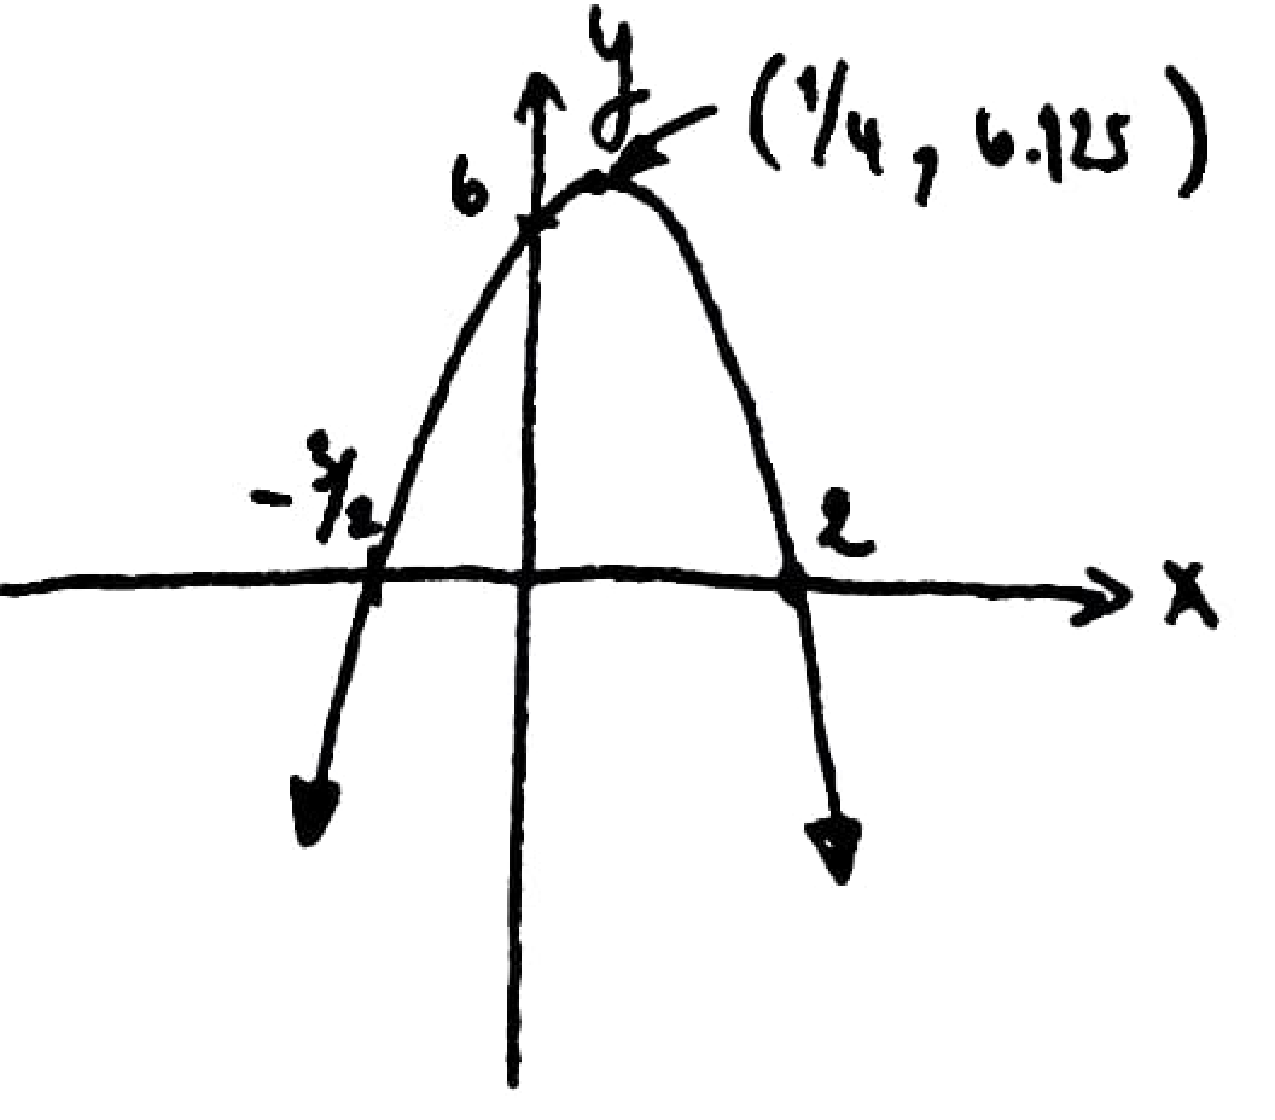
\includegraphics[height = 4cm]{geometryandcalculus/parabolasketch.pdf}
		\caption{Sketch of the function $-2x^2 + x + 6$.}
	\end{figure}
\end{exmp}

We can also determine the amount of roots by just looking at the $y$-value of the vertex point, given by \cref{eq:parabola_y_vertex}, and the direction of the parabola. But it's more computationally expensive than the determinant method which says,
\begin{displayquote}
	A parabola has no roots if $b^2 - 4ac < 0$, one root if $b^2 - 4ac = 0$, and two roots if $b^2 - 4ac > 0$.
\end{displayquote}
This is a direct result of the quadratic formula: $x = \frac{- b \pm \sqrt{b^2 - 4ac}}{2a}$ only have real solution if the terms in the root, $b^2 - 4ac$, is positive.

\subsection{Shape of cubics}

Cubics are third order polynomials
\begin{equation}
	f(x) = ax^3 + bx^2 + cx + d.
\end{equation}
It's one of the many family of function that can contain more than one stationary point. The $x$ coordinate of the stationary points can be found by using the same method as earlier.
\begin{align}
	\odv{f(x)}{x} &= \odv*{ax^3 + bx^2 + cx + d}{x} \\
				  &= 3ax^2 + 2bx + c,
\end{align}
in which
\begin{align}
	\odv{f(x)}{x}_{x = x_0} = 0 &= 3ax_0^2 + 2bx_0 + c \\
	x_0 &= \frac{- 2b \pm \sqrt{(2b)^2 - 4(3a)(c)}}{2(3a)} \\
		&= \frac{- 2b \pm 2\sqrt{b^2 - 3ac}}{6a} \\
		&= \frac{- b \pm \sqrt{b^2 - 3ac}}{3a}. \label{eq:cubic_vertex_position-x}
\end{align}
By the terms under the root, a cubic has no stationary point if $\frac{b^2 - 3ac}{3a} < 0$, one if $\frac{b^2 - 3ac}{3a} = 0$, and two if $\frac{b^2 - 3ac}{3a} > 0$.

The function $f(x)$ intersects the $y$ axis when $x = 0$:
\begin{equation}
	f(0) = a(0)^3 + b(0)^2 + c(0) + d = d;
\end{equation}
thus, the $y$ intercept is at $(0, d)$. For the $x$-intercept, again, there is no tool in calculus that can be used to find the exact root. So, you'd just have to either factor the function, or use the very lengthy cubic formula.
\begin{equation}
	\begin{gathered}
		x = \sqrt[3]{q + \sqrt{q^2 + (r - p^2)^3}} + \sqrt[3]{q - \sqrt{q^2 + (r - p^2)^3}} + p
	\end{gathered}
\end{equation}
where
\begin{equation}
	p = -\frac{b}{3a}, \quad q = p^3 + \frac{bc - 3ad}{6a^2} \mathand r = \frac{c}{3a}.
\end{equation}

% Insert examples here

Another topic that I'd like to discuss is the amount of root of cubics. Normally, we would use factorization to determine the amount. From the shape of the cubic, one side shoots of to positive infinity, and the other, negative infinity. And by continuity, it must intersect the $x$ axis somewhere inbetween and create a root. Therefore, all cubics must have at least one root over the reals. But what if we want to know whether it has a second or third roots or not? We can just look at the amount and the position of the stationary point, given by \cref{eq:cubic_vertex_position-x}.

A key feature of stationary points is that they indicate where a function changes direction. If a function is increasing and then begins to decrease, there must be a stationary point marking this transition. So, if a function lacks a stationary point, and one end tends toward positive infinity while the other falls to negative infinity, we can conclude the function is always either increasing or decreasing. Once the function intersects the $x$-axis to form a root, it cannot turn back to create another root.

A cubic with zero stationary points ($\frac{b^2 - 3ac}{3a} < 0$) are such kind of function. One side goes to infinity, and the other, negative infinity. Since it has no stationary point, it must only have one root. One such example is the function $f(x) = x^3 + x^2 + x$, plotted in \cref{fig:cubic_no_vertex}.

\begin{figure}[t]
	\centering
	\begin{subfigure}[t]{0.3\textwidth}
		\centering
		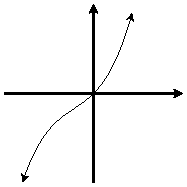
\includegraphics{geometryandcalculus/cubic_novertex.pdf}
		\caption{$x^3 + x^2 + x$: No vertex}
		\label{fig:cubic_no_vertex}
	\end{subfigure}
	\begin{subfigure}[t]{0.3\textwidth}
		\centering
		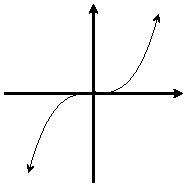
\includegraphics{geometryandcalculus/cubic_onevertex.pdf}
		\caption{$x^3$: One vertex}
		\label{fig:cubic_one_vertex}
	\end{subfigure}
	\caption{Cubics with zero and one vertex}
\end{figure}

Similarly, cubics with only one stationary point ($\frac{b^2 - 3ac}{3a} = 0$) only have one root. Illustrated in \cref{fig:cubic_one_vertex}, the stationary point must be an inflection point, as it cannot represent a local maximum or minimum. This is due to the behavior of the function, which extends toward both positive and negative infinity. If the stationary point were a local maximum or minimum, it would turn into a parabola, and thus needs another point to reverse its direction again to be a cubic. Hence, cubic functions with only one stationary point have just one root.

\begin{figure}[ht]
	\centering
	\begin{subfigure}[t]{0.3\textwidth}
		\centering
		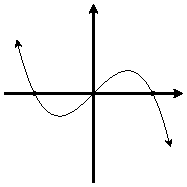
\includegraphics[]{geometryandcalculus/cubic_twovertex_threeroots.pdf}
		\caption{$x^3 + x$: Three roots}
		\label{fig:cubic_two_vertices_threeroots}
	\end{subfigure}
	\begin{subfigure}[t]{0.3\textwidth}
		\centering
		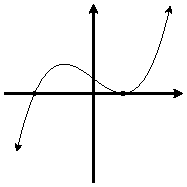
\includegraphics[]{geometryandcalculus/cubic_twovertex_tworoots.pdf}
		\caption{$x^3 - \frac{3}{4}x + \frac{1}{4}$: Two roots}
		\label{fig:cubic_two_vertices_tworoots}
	\end{subfigure}
	\begin{subfigure}[t]{0.3\textwidth}
		\centering
		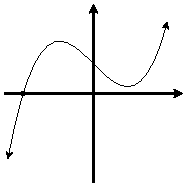
\includegraphics[]{geometryandcalculus/cubic_twovertex_oneroot.pdf}
		\caption{$x^3 - x$: One root}
		\label{fig:cubic_two_vertices_oneroot}
	\end{subfigure}
	\caption{Two vertices cubics with varying amount of roots}
	\label{fig:cubic_two_vertices}
\end{figure}

For cubics with two vertex, one of those must be a local maximum, the other, a local minimum. The amount of roots can be directly determined by the position of these points. A cubic will have three roots if the vertex aren't on the same side of the $x$ axis, it must have three roots, illustrated in \cref{fig:cubic_two_vertices_threeroots}. If one of the vertex is at $y = 0$, then it has two roots; one of them being the vertex itself, illustrated in \cref{fig:cubic_two_vertices_tworoots}. If both vertices are on the same side, then it must have only one root; illustrated in \cref{fig:cubic_two_vertices_oneroot}. It is left as an exercise for the reader to find the position of vertices of the cubics given in \cref{fig:cubic_two_vertices}

\subsection{Optimization problems}

The method of finding local maxima, minima, and inflection points are very useful for sketching graphs. Are there any real life applications to this? The answer is in optimization.

\textbf{Optimization} is about finding the best solution for a problem. What's the best time to harvest the crop? What's the best placement for an air conditioner? What's the best way to make profit?, etc. These problems are all about finding the maximum values of some variables. That's exactly what our tools have been able to do: finding the maxima and minima of some functions. Thus, I'd like to discuss about some applications of maxima and minima on some physical problems. \index{optimization problems}

\begin{wrapfigure}{r}{0.3\textwidth}
	\centering
	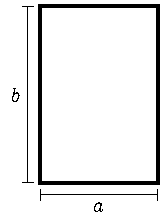
\includegraphics{geometryandcalculus/optimization_rectangle_area_fixed_perimeter.pdf}
	\caption{A rectangle for optimization}
	\label{fig:optimization_rectangle_area_fixed_perimeter}
\end{wrapfigure}
\paragraph{Classic maximum area problem.} Given a rope length $L$, what's the maximum rectangular area that this rope can enclose?

To solve this problem, we start by constructing our rectangle. Drawn in \cref{fig:optimization_rectangle_area_fixed_perimeter}, the perimeter of a rectangle is given by $2(a + b) = L$. Without loss of generality, let side $a$ has length $l$. Thus,
\begin{align}
	2(l + b) &= L \\
	b &= \frac{L}{2} - l
\end{align}
The area of the rectangle, which is a function of $l$, $A(l)$ is then
\begin{equation}
	A(l) = a \times b = l\ab(\frac{L}{2} - l) = -l^2 + l\frac{L}{2}.
\end{equation}
Since this function is a parabola, its stationary point must be the local maxima, and must also be the global maxima. This point is where our function is the highest. It can be found by using the derivative w.r.t. $l$.
\begin{equation}
	\odv*{A(l)}{l} = -2l + \frac{L}{2}
\end{equation}
Using the same argument as earlier, we want to find the point $l_0$ where $\odv*{A(l)}{l}_{l = l_0} = 0$:
\begin{align}
	0 &= - 2l_0 + \frac{L}{2} \\
	l_0 &= \frac{L}{4};
\end{align}
thus, the maximum $A(l)$ is
\begin{equation}
	A\ab(\frac{L}{4}) = -\ab(\frac{L}{4})^2 + \ab(\frac{L}{4})\frac{L}{2} = \frac{L^2}{16}
\end{equation}
Funnily enough, the maximum area that a perimeter length $L$ can increase is also a parabola $\frac{1}{16}L^2$.

\paragraph{Modified maximum area problem.} Given a fence length $L$. What's the maximum area that I can enclose, given that one of the sides doesn't need any fence?

If our rectangle has sides $a$ and $b$, and one side doesn't need a fence, without loss of generality, the perimeter is $a + 2b = L$. If $a = l$, then $b = \frac{L - l}{2}$. The area of the rectangle then becomes
\begin{equation}
	A(l) = a \times b = l\ab(\frac{L - l}{2}) = - \frac{1}{2}l^2 + \frac{L}{2}l. 
\end{equation}
Using the same argument,
\begin{align}
	\odv*{A(l)}{l} &= -l + \frac{L}{2} \\
	\odv*{A(l)}{l}_{l = l_0} = 0 &= -l_0 + \frac{L}{2} \\
	l_0 &= \frac{L}{2},
\end{align}
and
\begin{align}
	A(l_0) = -\frac{1}{2}\ab(\frac{L}{2})^2 + \frac{L}{2}\ab(\frac{L}{2}) = \frac{3}{8}L^2.
\end{align}

\paragraph{Volume of a box.} Let's say you have a paper size $a \times b$, shown in \cref{fig:optimization_box_volume_unfold}. If you want to fold it up into a box without a closing top by cutting a square size $x$ on each corner, shown in \cref{fig:optimization_box_volume_folded}, find the maximum volume that the box can enclose.

\begin{figure}[ht]
	\centering
	\begin{subfigure}[b]{0.51\textwidth}
		\centering
		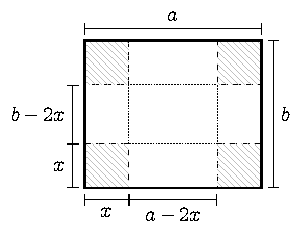
\includegraphics[]{geometryandcalculus/optimization_box_volume_unfold.pdf}
		\caption{Unfolded. The gray part is cut out.}
		\label{fig:optimization_box_volume_unfold}
	\end{subfigure}
	\begin{subfigure}[b]{0.43\textwidth}
		\centering
		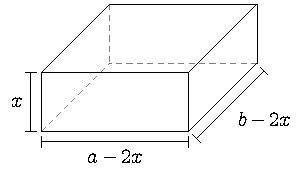
\includegraphics[]{geometryandcalculus/optimization_box_volume_folded.pdf}
		\caption{Folded}
		\label{fig:optimization_box_volume_folded}
	\end{subfigure}
	\caption{Box volume optimization}
\end{figure}

Shown in \cref{fig:optimization_box_volume_unfold}, if we cut out a square sidelength $x$ from all corners, then the sidelength of the final box will be $a - 2x$, $b - 2x$, and $x$. The volume $V(x)$, is then
\begin{equation}
	V(x) = x(a - 2x)(b - 2x) = 4x^3 + (- 2a - 2b)x^2 + (ab)x
\end{equation}
This function is a cubic, and we can use \cref{eq:cubic_vertex_position-x} to find the $x$ coordinate of the vertex.
\begin{align}
	x_0 &= \frac{- (- 2a - 2b) \pm \sqrt{(- 2a - 2b)^2 - 3(4)(ab)}}{3(4)} \\
		&= \frac{2a + 2b \pm \sqrt{4a^2 + 4b^2 - 4ab}}{12} \\
		&= \frac{a + b \pm \sqrt{a^2 + b^2 - ab}}{6}
\end{align}
If $a^2 + b^2 - ab = 0$, there's only one stationary point at $x_0 = \frac{a + b}{6}$, which is an inflection point. Otherwise, it must have two stationary points. Since the leading coefficient of $V(x)$ is positive, $V(x)$ must approach negative infinity when $x$ approaches infinity. Meaning that, the highest local maxima is on the right vertex; thus, we select the negative root:
\begin{equation}
	x_0 = \frac{a + b - \sqrt{a^2 + b^2 - ab}}{6}.
\end{equation}
The full solution is left out due to arithmetical tediousness. It'd be better if you just plug in the numbers.

\section{Tangent to a curve}

In this section, I'll show you how to find a line that's tangent to a curve. But to do it the traditional way would be a bit boring, as it's quite dry and actually doesn't help us with graph sketching at all. So, I shall introduce it via the Newton-Raphson's root finding algorithm; as it's an algorithm that directly takes advantage of the line tangent to a function, and it shows up in many places. So much so that it exists inside the core of the fast square root algorithm which is implemented in every computer.

\subsection{Newton-Raphson method}

Polynomials appears everywhere. Most of the time, you're required to find its root. But it might come as a surprise for you that it is \emph{impossible} to find a general for finding the root of polynomials with degrees higher than four. This is a direct consequence of Galois theory\footnote{The Galois theory is a profound result from abstract algebra. You would usually learn in graduate mathematics, but if you want to just scratch the surface, I found a video by \emph{Math Visualized}, on \emph{Galois Theory Explained Simply} \cite{galois-explained-2020}, that explains it quite clearly. Still, I need to watch it a couple of times before understanding it.}, one of the most important theory in abstract algebra. So most of the time, we resort to root approximation methods.

The root approximation method which is relevant to calculus is the Newton-Raphson's root finding algorithm. I'd try to explain this algorithm has much as I can, but I think it's better if you see it.

The Newton-Raphson algorithm takes advantage of slopes descent. Let's say you want to approximate the root of $f(x)$. You put down a random guess, say $x_1$. If that point is a root, $f(x_1) = 0$. If its not, the root is either above ($f(x_1) < 0$) the point or under ($f(x_1) > 0$). What you do next is that you draw a line tangent to the function $f(x)$ at $x = x_1$ and let it cross the $x$-axis, shown in \cref{fig:newton-raphson-method}. Intuitively, the tangent line will intersect the $x$-axis at $x_2$ where $x_2$ should hopefully be closer to the root. Our new guess will then be $(x_2, f(x_2))$. We then repeat this method until the approximation are satisfactory.

Here, I shall use the Newton-Raphson root finding algorithm as a way to introduce you about how calculus can be further applied to geometry.

\begin{figure}[ht]
	\centering
	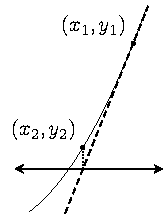
\includegraphics{geometryandcalculus/newton-raphson-method.pdf}
	\caption{Newton-Raphson's method illustrated}
	\label{fig:newton-raphson-method}
\end{figure}

The first part of the Newton-Raphson method is to be able to find the tangent to a curve. Let's first start with a line equation
\begin{equation}
	y = mx + c.
\end{equation}
If my first guess is on the point $(x_1, f(x_1))$, the line that passes through that point and tangent to $f(x)$ is
\begin{equation}
	y = \odv{f(x)}{x}_{x = x_1}x + c.
\end{equation}
where $m = \odv{f(x)}{x}_{x = x_1}$. And $c$ is the intersection with the $x$ axis.

But we don't have to actually find $c$. For a line tangent to a curve, we just want to move the line from the origin to the tangent point $(x_1, f(x_1))$. To move the line to the right by $x_1$ units, we substitute $x$ with $x - x_1$, and to shift it up by $y_1$, substitute $y$ with $y - y_1$. Thus, the line equation turns into
\begin{align}
	y - y_1 &= (x - x_1)\odv{f(x)}{x}_{x = x_1} \\
	y - f(x_1) &= (x - x_1)\odv{f(x)}{x}_{x = x_1}.
\end{align}
For simplicity of notation, I shall let $\mdif{x}f(x_1)$ represent $\odv{f(x)}{x}$:
\begin{equation}
	y - f(x_1) = (x - x_1)\mdif{x}f(x_1).
\end{equation}

Then, Newton-Raphson method tells us that the intersection between the tangent line and the $x$ axis is what our next guess, $x_2$, should be. It can be easily evaluated by setting $y = 0$.
\begin{align}
	0 - f(x_1) &= (x_2 - x_1)\mdif{x}f(x_1) \\
	x_2 &= x_1 - \frac{f(x_1)}{\mdif{x}f(x_1)}
\end{align}
Generally, we can repeat this forever. Thus,
\begin{equation}
	x_{n + 1} = x_n - \frac{f(x_n)}{\mdif{x}f(x_n)} \label{eq:newton-raphson-method}
\end{equation}
a recurrence relation for finding roots of functions. Notice that we don't even need to know the $y$ value for this algorithm to work. And that's the beauty of it.

Let's use this root finding method to approximate $\sqrt{2}$, which is the root of the polynomial $x^2 - 2 = 0$. Since the derivative of $x^2 - 2$ is $2x$, Newton-Raphson method (\cref{eq:newton-raphson-method}) gives
\begin{align}
	x_{n + 1} &= x_n - \frac{x_n^2 - 2}{2x_n} \\
			  &= \frac{x_n^2 + 2}{2x_n}.
\end{align}
Since $\sqrt{2} \approx 1.414213\dots$, let's use $x_1 = 1$ as our first guess.
\begin{align}
	x_2 &= \frac{x_1^2 + 2}{2x_1} \\
		&= \frac{1^2 + 2}{2(1)} = 1.5,
\end{align}
which is closer to $1.41$ than our first guess. Next,
\begin{align}
	x_3 &= \frac{x_2^2 + 2}{2x_2} \\
		&= \frac{1.5^2 + 2}{2(1.5)} = 1.4166\dots,
\end{align}
which is off by just a $0.2\%$ error. By the forth iteration, we get $1.414215\dots$, which is off by a mere $0.0002\%$. And we can stop here.

\subsection{Numerical version of the Newton-Raphson method}

For a function that you can't find a derivative, or you're just too lazy to explicitly find the derivative, you can turn the Newton-Raphson method into a numerical method via the definition of derivative\cref{eq:newton-raphson-method}.
\begin{align}
	x_{n + 1} &= x_n - \frac{f(x_n)}{\lim_{h \appr 0}\frac{f(x_n + h) - f(x_n)}{h}} \\
			  &= x_n - \lim_{h \appr 0}\frac{f(x_n)h}{f(x_n + h) - f(x_n)}.
\end{align}
Computationally, we can set $h$ to any arbitrarily small values: $0.01$ for example. If you have some experiences with coding, this can be easily implemented by using a \texttt{for} loop. Here's some python code that I've written to do just that. Just put in the function in \texttt{def f(x):} block, put the amount of iteration in \texttt{iterationCount}, your first guess in \texttt{firstGuess}, and the value of $h$ in \texttt{derivativeStep}. If you have some experiences, I highly encourage you to tinker around.

\begin{minted}{python}
import matplotlib.pyplot as plt
import math

def f(x):  # Insert function here
    return x**3 - 2 * x + 1

iterationCount = 10  # Amount of iteration
firstGuess = -2  # First guess
derivativeStep = 0.01  # For calculating the method of increments
approximationList = [float(firstGuess)]  # List of approximations
for i in range(iterationCount):
    diff = (
        f(approximationList[i] + derivativeStep) - f(approximationList[i])
    ) / derivativeStep  # Finding the derivative at a certain point
    nextGuess = (
        approximationList[i] - f(approximationList[i]) / diff
    )  # Newton-Raphson's method
    approximationList.append(nextGuess)  # Add next guess to the list of approximations

print(approximationList)  # Print out the list of approximations
fig, axes = plt.subplots()  # Initiate plot
axes.plot(list(range(iterationCount + 1)), approximationList)  # Plotting
axes.set_xlabel("Iteration")  # Setting the x-axis label
axes.set_ylabel("Guess")  # Setting the y-axis label
plt.show()  # Showing the plot
\end{minted}

\section{Normal lines}
\label{sec:normal-lines}

Alongside the tangent line, there is another line that we're interested in: the normal line, a line that's perpendicular to the tangent. It's actually pretty simple to solve. By analytical geometry, if two lines are perpendicular to each other, the product of their slope must be $-1$.

If the slope of tangent is $m_T$ and the normal is $m_N$,
\begin{align}
	m_T \times m_N &= -1 \\
	m_N &= -\frac{1}{m_T}.
\end{align}
Since the slope of the tangent at a point $(x_0, f(x_0))$ is $\mdif{x}f(x_0)$,
\begin{equation}
	m_N = -\frac{1}{\mdif{x}f(x_0)}.
\end{equation}
The normal line equation can then be formed by translating the line with slope $m_N$ to the point $(x_0, f(x_0))$:
\begin{equation}
	y - f(x_0) = -\frac{x - x_0}{\mdif{x}f(x_0)}.
\end{equation}

\section{Arc length of functions}

Before we wrap off this chapter, here's a fun geometrical problem to think about. Given a function $f(x)$, what's the length of the line drawn by the function from $a$ to $b$? Illustrated in \cref{fig:arclength}, the total arc length $s$ can be subdivided into smaller arc lengths $\odif{s}$ that we can sum up. How? Integrals. 

\begin{figure}[ht]
	\centering
	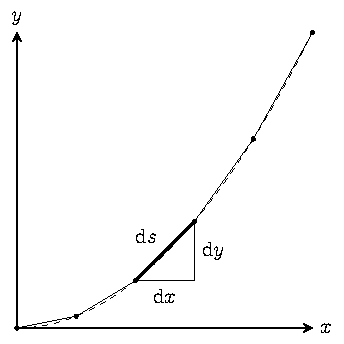
\includegraphics{geometryandcalculus/arclength.pdf}
	\caption{Arc length calculation}
	\label{fig:arclength}
\end{figure}

The total arc length $s$ of the function $f(x)$ from $a$ to $b$ is just
\begin{equation}
	\int_{a}^{b}\odif{s}
\end{equation}
By the Pythagorean theorem $\odif{s} = \sqrt{\odif{x}^2 + \odif{y}^2}$. Can we plug this directly into the integral? Of course we can:
\begin{equation}
	s = \int_{x = a}^{x = b}\sqrt{\odif{x}^2 + \odif{y}^2}.
\end{equation}
Factorizing $\odif{x}$ out of the square root would yield an integral
\begin{align}
	\int_{x = a}^{x = b}\sqrt{\odif{x}^2 + \odif{y}^2} &= \int_{x = a}^{x = b}\sqrt{1 + \ab(\odv{y}{x})^2}\odif{x} \\
													   &= \int_{x = a}^{x = b}\sqrt{1 + \ab(\odv{f(x)}{x})^2}\odif{x}.
\end{align}
Simply plug in the derivative of $f(x)$ and evaluate the integral, and you would get the arclength.

